\documentclass[aspectratio=169, table]{beamer}

\usepackage[utf8]{inputenc}
\usepackage{listings} 

\usetheme{Pradita}

\subtitle{MTI104 - IT Services}

\title{Session-13:\\\LARGE{The Service Desk\\}}
\date[Serial]{\scriptsize {PRU/SPMI/FR-BM-18/0222}}
\author[Pradita]{\small{\textbf{Alfa Yohannis}}}

\begin{document}

\frame{\titlepage}

\begin{frame}{Service Desk in ITIL Framework}
	\begin{itemize}
		\item The service desk is integral to the ITIL framework.
		\item Most ITIL implementations prioritize the service desk.
		\item It is a people-led practice, different from process-led practices.
		\item Acts as the face of the service provider organization.
		\item Single point of contact for users, suppliers, and customers.
		\item Example: Calling the service desk for mobile phone billing issues.
	\end{itemize}
\end{frame}

\begin{frame}{Importance of the Service Desk}
	\begin{itemize}
		\item Becomes the face of the service provider organization.
		\item Professional etiquette is crucial for service desk representation.
		\item Organization's image depends on the service desk interaction.
		\item Poor service desk interaction can damage the provider’s reputation.
		\item Service desk is included in the ITIL Foundation exam.
		\item Key practice with 3-4 questions expected in the exam.
	\end{itemize}
\end{frame}

\begin{frame}{Service Desk in ITIL Framework}
	\begin{itemize}
		\item In ITIL, service desk was once a function, now a practice.
		\item No distinction between processes and functions in ITIL 4.
		\item Responsible for defined deliveries and set objectives.
		\item Purpose: Capture demand for incident resolution and service requests.
		\item Acts as the entry point and single point of contact for users.
		\item First line of support, with escalation to second and third lines.
	\end{itemize}
\end{frame}

\begin{frame}{Why a Service Desk?}
	\begin{itemize}
		\item Previously, no need for service desks in small organizations.
		\item Direct rapport with technical teams was sufficient.
		\item Increased IT end users require structured support.
		\item Service desk channels triggers and prioritizes incidents.
		\item Facilitates the proper routing of incidents to the right teams.
		\item Service desk is now essential for IT service management.
	\end{itemize}
\end{frame}

\begin{frame}{Benefits of Having a Service Desk}
	\begin{itemize}
		\item Improves accessibility to IT staff for users and customers.
		\item Optimizes usage of IT resources.
		\item Enhances customer service and excitement.
		\item Provides faster turnaround on service requests.
		\item Optimizes the cost of providing IT support.
		\item Entry-level employees reduce operational costs.
		\item Provides a win-win situation for all stakeholders.
	\end{itemize}
\end{frame}

\begin{frame}{Business and Technology}
	\begin{itemize}
		\item Service desk was originally called a help desk.
		\item Help desk: single point of contact for users to report issues.
		\item ITIL expanded service desk to support suppliers and customers.
		\item A mature service desk manages 50% of overall tickets.
		\item Service desk handles various functions, including first-line support.
		\item Success due to use of less skilled, cost-effective resources.
	\end{itemize}
\end{frame}

\begin{frame}{Evolution of the Service Desk}
	\begin{itemize}
		\item IT became a partner in decision-making with businesses.
		\item Service desk reimagined for wider business functions.
		\item Not limited to IT issues, but also janitorial, electrical, etc.
		\item Modern service desks handle multiple types of issues.
		\item Specialized agents handle different types of requests.
		\item Channels to reach the service desk have evolved over time.
	\end{itemize}
\end{frame}

\begin{frame}{Channels to Reach Service Desk}
	\begin{itemize}
		\item Walk-ins: Physical visits to the service desk were common.
		\item Telephones: Most popular means, but can be time-consuming.
		\item Emails: Easier for non-urgent issues, but slower than calls.
		\item Chatting: Non-intrusive and efficient; allows multitasking.
		\item Portals: Self-help tools for users to log incidents directly.
		\item Messaging: Modern options like WhatsApp and SMS are emerging.
	\end{itemize}
\end{frame}

\begin{frame}
	\frametitle{Social Media in Service Desk}
	\begin{itemize}
		\item Communication channels taken over for service provider organizations
		\item Popular channels: Twitter and Facebook
		\item Users interact with service desk by raising issues via social media
		\item Responses sent back through the same channels
		\item Public nature of interactions discourages use of social media
		\item Interactions not private, on public pages instead
		\item Feature available but not always preferred by users
	\end{itemize}
\end{frame}

\begin{frame}
	\frametitle{Service Desk Structures}
	\begin{itemize}
		\item Organizations have varying service desk structures
		\item Structures driven by strategy
		\item Traditional organizations: hierarchical structure
		\item Start-ups and new age organizations: flat structure
		\item Structure impacts value creation and resource utilization
		\item Core objectives dictate service desk structuring
		\item Three common types: Local, Centralized, Virtual
	\end{itemize}
\end{frame}

\begin{frame}{Typical support lines in a DevOps organization}
	 \frametitle{Typical support lines in a DevOps organization}
\begin{center}
	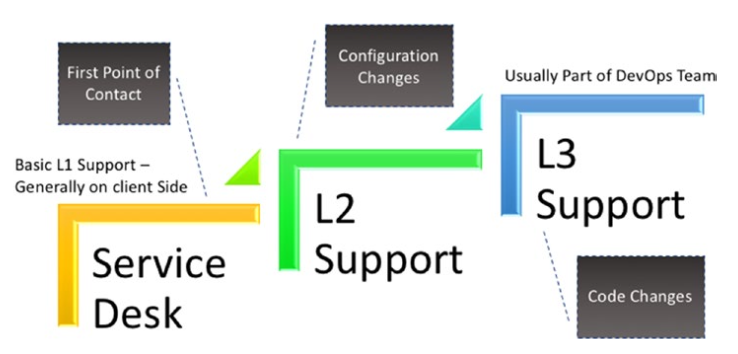
\includegraphics[width=0.8\linewidth]{images/image-01.png}
\end{center}
\end{frame}

\begin{frame}
	\frametitle{Local Service Desk}
	\begin{itemize}
		\item Limited boundary, serves a subset of the overall function
		\item Specific to an office, location, or region
		\item Examples: Bangalore, Sydney, Zurich service desks
		\item Users, technical teams, suppliers reach out to their respective local desk
		\item Advantages: better understanding due to common language, culture
		\item Customized service for VIP users
		\item Increased customer satisfaction
	\end{itemize}
\end{frame}

\begin{frame}{Local service desk}
	 \frametitle{Local service desk}
\begin{center}
	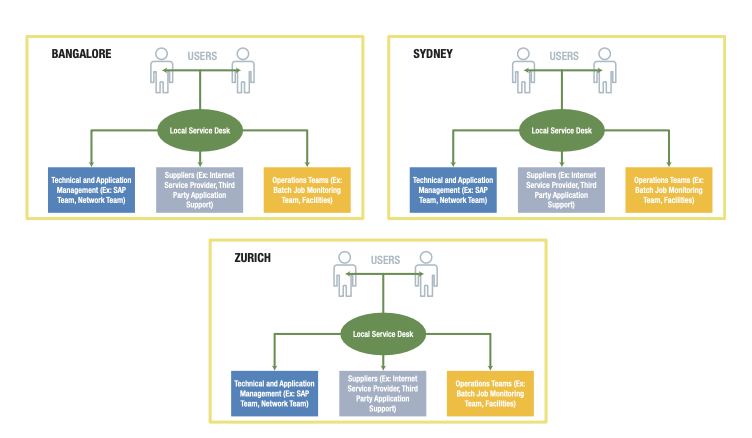
\includegraphics[width=0.8\linewidth]{images/image-02.png}
\end{center}
\end{frame}

\begin{frame}
	\frametitle{Disadvantages of Local Service Desk}
	\begin{itemize}
		\item Expensive due to duplication of infrastructure, applications
		\item Call volumes may not justify existence of local desks
		\item Lack of standardized processes and tools
		\item Differential treatment possible due to non-standardization
	\end{itemize}
\end{frame}

\begin{frame}
	\frametitle{Centralized Service Desk}
	\begin{itemize}
		\item Most popular structure among organizations
		\item Single service desk at a strategic location
		\item Example: Centralized desk serving Bangalore, Sydney, Zurich
		\item Centralized technical teams manage respective technologies
		\item Provides a single point of contact for all end users
		\item Cost-effective compared to local service desks
		\item Easier to achieve standardization
	\end{itemize}
\end{frame}

\begin{frame}{Centralized service desk}
	 \frametitle{Centralized service desk}
\begin{center}
	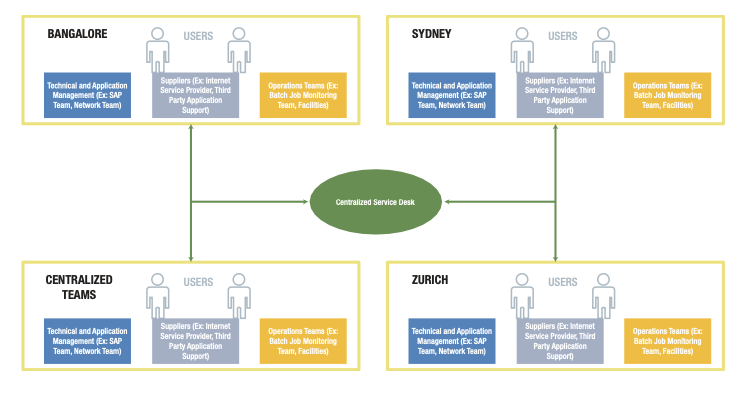
\includegraphics[width=0.8\linewidth]{images/image-03.png}
\end{center}
\end{frame}

\begin{frame}
	\frametitle{Advantages of Centralized Service Desk}
	\begin{itemize}
		\item Economical due to single setup
		\item Optimized resource utilization
		\item Better management overview of performance
		\item Centralized processes, procedures, standards
	\end{itemize}
\end{frame}

\begin{frame}
	\frametitle{Disadvantages of Centralized Service Desk}
	\begin{itemize}
		\item Loss of local flavor, language, culture
		\item Some users prefer proximity and personal touch
		\item Centralized service may not satisfy all locations
	\end{itemize}
\end{frame}

\begin{frame}
	\frametitle{Virtual Service Desk}
	\begin{itemize}
		\item Centralized service desk achieved through technology
		\item Service desk agents operate from different global locations
		\item Common Service Knowledge Management System (SKMS) used
		\item Seamless integration of disjointed parts into a single unit
		\item Off-shoring, near-shoring, and outsourcing of service desks
		\item Follow-the-sun model for 24/7 global support
		\item Specialized service desks based on expertise
	\end{itemize}
\end{frame}

\begin{frame}{Virtual service desk}
	 \frametitle{Virtual service desk}
\begin{center}
	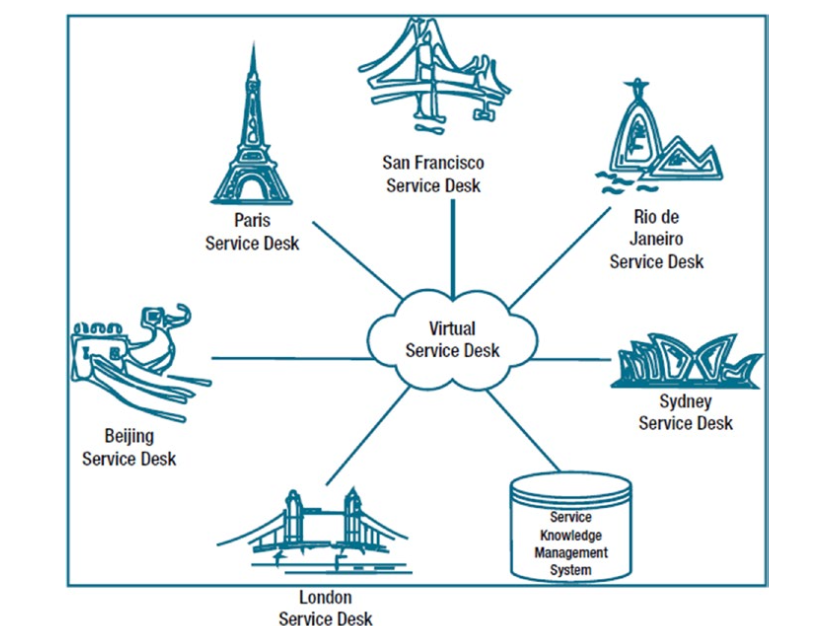
\includegraphics[width=0.5\linewidth]{images/image-04.png}
\end{center}
\end{frame}

\begin{frame}
	\frametitle{Advantages of Virtual Service Desk}
	\begin{itemize}
		\item Resilient with multiple service desks
		\item Cost-effective, especially with home-working professionals
		\item No infrastructure costs for agents working from home
		\item Avoids additional wage costs for working beyond set hours
	\end{itemize}
\end{frame}

\begin{frame}
	\frametitle{Disadvantages of Virtual Service Desk}
	\begin{itemize}
		\item Challenging alignment of processes, procedures, and language
		\item Coordination between virtual and technical teams can be difficult
		\item Possible differences in service quality across locations
		\item Requires extensive management efforts and automation
	\end{itemize}
\end{frame}

\begin{frame}
	\frametitle{Qualities Expected from Service Desk Staff}
	\begin{itemize}
		\item Communication and soft skills are essential
		\item Service desk is the first point of contact for users
		\item Staff must be calm and assure users during incidents
		\item Frequent communication with engineers for updates
		\item Technical orientation is necessary for resolving issues
		\item Ability to prioritize and escalate incidents correctly
		\item Probing users effectively for accurate and quick resolutions
	\end{itemize}
\end{frame}

\begin{frame}
	\frametitle{Empathy and Social Intelligence}
	\begin{itemize}
		\item Empathy is crucial when dealing with frustrated users
		\item Understanding users' problems is the first step
		\item Social intelligence can separate excellent staff from the rest
		\item Example: Amazon service desk agent's empathetic response
		\item Empathy builds trust and customer satisfaction
	\end{itemize}
\end{frame}

\begin{frame}
	\frametitle{Service Desk and Automation}
	\begin{itemize}
		\item Automation is increasingly integrated into service desks
		\item Reduces service costs while maintaining service levels
		\item Replaces repetitive tasks traditionally done by humans
		\item Capital investment in automation leads to long-term benefits
		\item IVR systems often replace initial human interaction
		\item Automation is beneficial if it provides correct answers
		\item Some processes are better automated, but human touch remains vital
	\end{itemize}
\end{frame}

\begin{frame}
	\frametitle{Multiple Choice Question}
	
	Under which of the SVC activities does the service desk play a major role?
	
	\begin{enumerate}[A.]
		\item Obtain/Build
		\item Design and Transition
		\item Improve
		\item Engage
	\end{enumerate}
	
\end{frame}


\end{document}
